%%%%%%%%%%%%%%%%%%%%%%%%%%%%%%%%%%%%%%%%%%%%%%%%%%%%%%%%%%%%%%%%%%%%%%%%%%%%%%%%%%%%%%%%%%%%%%%%%%%%%%%%%%%%%%%%%%%%%%%%%%%%%%%%%%%%%%%%%%%%%%%%%%%%%%%%%%%%%%%%%%%
% Written By Michael Brodskiy
% Class: Electricity & Magnetism
% Professor: D. Wood
%%%%%%%%%%%%%%%%%%%%%%%%%%%%%%%%%%%%%%%%%%%%%%%%%%%%%%%%%%%%%%%%%%%%%%%%%%%%%%%%%%%%%%%%%%%%%%%%%%%%%%%%%%%%%%%%%%%%%%%%%%%%%%%%%%%%%%%%%%%%%%%%%%%%%%%%%%%%%%%%%%%

\documentclass[12pt]{article} 
\usepackage{alphalph}
\usepackage[utf8]{inputenc}
\usepackage[russian,english]{babel}
\usepackage{titling}
\usepackage{amsmath}
\usepackage{graphicx}
\usepackage{enumitem}
\usepackage{amssymb}
\usepackage[super]{nth}
\usepackage{everysel}
\usepackage{ragged2e}
\usepackage{geometry}
\usepackage{multicol}
\usepackage{fancyhdr}
\usepackage{cancel}
\usepackage{siunitx}
\usepackage{physics}
\usepackage{tikz}
\usepackage{mathdots}
\usepackage{yhmath}
\usepackage{cancel}
\usepackage{color}
\usepackage{array}
\usepackage{multirow}
\usepackage{gensymb}
\usepackage{tabularx}
\usepackage{extarrows}
\usepackage{booktabs}
\usepackage{lastpage}
\usetikzlibrary{fadings}
\usetikzlibrary{patterns}
\usetikzlibrary{shadows.blur}
\usetikzlibrary{shapes}

\geometry{top=1.0in,bottom=1.0in,left=1.0in,right=1.0in}
\newcommand{\subtitle}[1]{%
  \posttitle{%
    \par\end{center}
    \begin{center}\large#1\end{center}
    \vskip0.5em}%

}
\usepackage{hyperref}
\hypersetup{
colorlinks=true,
linkcolor=blue,
filecolor=magenta,      
urlcolor=blue,
citecolor=blue,
}


\title{Homework 2}
\date{September 28, 2023}
\author{Michael Brodskiy\\ \small Professor: D. Wood}

\begin{document}

\maketitle

\begin{enumerate}

  \item Six charges are arranged along the sides and corners of a square with sides of length L as shown. Calculate the magnitude and direction of the electric field at the origin. Use symmetry and superposition to make the calculation simple.

    \begin{center}
      \begin{figure}[H]
        \centering
        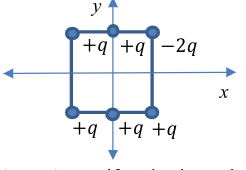
\includegraphics[width=.3\textwidth]{Figures/Figure2-1.png}
        \label{fig:1}
      \end{figure}
    \end{center}

    We know, by definition, that $\vec{F}=\vec{E}q$. Using the concepts we know about force, we know the following charges cancel out each other, as they are symmetric about the test charge at the origin:

    \begin{figure}[H]
      \centering
      \tikzset{every picture/.style={line width=0.75pt}} %set default line width to 0.75pt        

\begin{tikzpicture}[x=0.75pt,y=0.75pt,yscale=-1,xscale=1]
%uncomment if require: \path (0,430); %set diagram left start at 0, and has height of 430

%Shape: Grid [id:dp9511403020531122] 
\draw  [draw opacity=0] (225,103) -- (386,103) -- (386,264) -- (225,264) -- cycle ; \draw   (225,103) -- (225,264)(305,103) -- (305,264)(385,103) -- (385,264) ; \draw   (225,103) -- (386,103)(225,183) -- (386,183)(225,263) -- (386,263) ; \draw    ;
%Shape: Circle [id:dp026055485587581195] 
\draw  [color={rgb, 255:red, 74; green, 83; blue, 226 }  ,draw opacity=1 ][fill={rgb, 255:red, 74; green, 144; blue, 226 }  ,fill opacity=1 ][line width=1.5]  (219.5,103) .. controls (219.5,99.96) and (221.96,97.5) .. (225,97.5) .. controls (228.04,97.5) and (230.5,99.96) .. (230.5,103) .. controls (230.5,106.04) and (228.04,108.5) .. (225,108.5) .. controls (221.96,108.5) and (219.5,106.04) .. (219.5,103) -- cycle ;
%Shape: Circle [id:dp8849353673163125] 
\draw  [color={rgb, 255:red, 74; green, 83; blue, 226 }  ,draw opacity=1 ][fill={rgb, 255:red, 74; green, 144; blue, 226 }  ,fill opacity=1 ][line width=1.5]  (299.5,103) .. controls (299.5,99.96) and (301.96,97.5) .. (305,97.5) .. controls (308.04,97.5) and (310.5,99.96) .. (310.5,103) .. controls (310.5,106.04) and (308.04,108.5) .. (305,108.5) .. controls (301.96,108.5) and (299.5,106.04) .. (299.5,103) -- cycle ;
%Shape: Circle [id:dp7298663131993588] 
\draw  [color={rgb, 255:red, 74; green, 83; blue, 226 }  ,draw opacity=1 ][fill={rgb, 255:red, 74; green, 144; blue, 226 }  ,fill opacity=1 ][line width=1.5]  (379.5,103) .. controls (379.5,99.96) and (381.96,97.5) .. (385,97.5) .. controls (388.04,97.5) and (390.5,99.96) .. (390.5,103) .. controls (390.5,106.04) and (388.04,108.5) .. (385,108.5) .. controls (381.96,108.5) and (379.5,106.04) .. (379.5,103) -- cycle ;
%Shape: Circle [id:dp5118102160520555] 
\draw  [color={rgb, 255:red, 74; green, 83; blue, 226 }  ,draw opacity=1 ][fill={rgb, 255:red, 74; green, 144; blue, 226 }  ,fill opacity=1 ][line width=1.5]  (219.5,263) .. controls (219.5,259.96) and (221.96,257.5) .. (225,257.5) .. controls (228.04,257.5) and (230.5,259.96) .. (230.5,263) .. controls (230.5,266.04) and (228.04,268.5) .. (225,268.5) .. controls (221.96,268.5) and (219.5,266.04) .. (219.5,263) -- cycle ;
%Shape: Circle [id:dp9003932477737502] 
\draw  [color={rgb, 255:red, 74; green, 83; blue, 226 }  ,draw opacity=1 ][fill={rgb, 255:red, 74; green, 144; blue, 226 }  ,fill opacity=1 ][line width=1.5]  (299.5,263) .. controls (299.5,259.96) and (301.96,257.5) .. (305,257.5) .. controls (308.04,257.5) and (310.5,259.96) .. (310.5,263) .. controls (310.5,266.04) and (308.04,268.5) .. (305,268.5) .. controls (301.96,268.5) and (299.5,266.04) .. (299.5,263) -- cycle ;
%Shape: Circle [id:dp7160989607764205] 
\draw  [color={rgb, 255:red, 74; green, 83; blue, 226 }  ,draw opacity=1 ][fill={rgb, 255:red, 74; green, 144; blue, 226 }  ,fill opacity=1 ][line width=1.5]  (379.5,263) .. controls (379.5,259.96) and (381.96,257.5) .. (385,257.5) .. controls (388.04,257.5) and (390.5,259.96) .. (390.5,263) .. controls (390.5,266.04) and (388.04,268.5) .. (385,268.5) .. controls (381.96,268.5) and (379.5,266.04) .. (379.5,263) -- cycle ;
%Shape: Circle [id:dp693930431751913] 
\draw  [color={rgb, 255:red, 207; green, 248; blue, 28 }  ,draw opacity=1 ][fill={rgb, 255:red, 248; green, 231; blue, 28 }  ,fill opacity=1 ][line width=1.5]  (299.5,183) .. controls (299.5,179.96) and (301.96,177.5) .. (305,177.5) .. controls (308.04,177.5) and (310.5,179.96) .. (310.5,183) .. controls (310.5,186.04) and (308.04,188.5) .. (305,188.5) .. controls (301.96,188.5) and (299.5,186.04) .. (299.5,183) -- cycle ;
%Shape: Ellipse [id:dp5545063148136824] 
\draw  [color={rgb, 255:red, 208; green, 2; blue, 27 }  ,draw opacity=1 ] (305,68.5) .. controls (316.05,68.5) and (325,121.67) .. (325,187.25) .. controls (325,252.83) and (316.05,306) .. (305,306) .. controls (293.95,306) and (285,252.83) .. (285,187.25) .. controls (285,121.67) and (293.95,68.5) .. (305,68.5) -- cycle ;

% Text Node
\draw (217.5,103) node [anchor=east] [inner sep=0.75pt]    {$+q$};
% Text Node
\draw (217.5,263) node [anchor=east] [inner sep=0.75pt]    {$+q$};
% Text Node
\draw (305,94.1) node [anchor=south] [inner sep=0.75pt]    {$+q$};
% Text Node
\draw (305,271.9) node [anchor=north] [inner sep=0.75pt]    {$+q$};
% Text Node
\draw (392.5,263) node [anchor=west] [inner sep=0.75pt]    {$+q$};
% Text Node
\draw (392.5,103) node [anchor=west] [inner sep=0.75pt]    {$-2q$};


\end{tikzpicture}

      \caption{The Opposite Forces Negate Each Other}
      \label{fig:3}
    \end{figure}

    \begin{figure}[H]
      \centering
      \tikzset{every picture/.style={line width=0.75pt}} %set default line width to 0.75pt        

\begin{tikzpicture}[x=0.75pt,y=0.75pt,yscale=-1,xscale=1]
%uncomment if require: \path (0,430); %set diagram left start at 0, and has height of 430

%Shape: Grid [id:dp9511403020531122] 
\draw  [draw opacity=0] (225,103) -- (386,103) -- (386,264) -- (225,264) -- cycle ; \draw   (225,103) -- (225,264)(305,103) -- (305,264)(385,103) -- (385,264) ; \draw   (225,103) -- (386,103)(225,183) -- (386,183)(225,263) -- (386,263) ; \draw    ;
%Shape: Circle [id:dp026055485587581195] 
\draw  [color={rgb, 255:red, 74; green, 83; blue, 226 }  ,draw opacity=1 ][fill={rgb, 255:red, 74; green, 144; blue, 226 }  ,fill opacity=1 ][line width=1.5]  (219.5,103) .. controls (219.5,99.96) and (221.96,97.5) .. (225,97.5) .. controls (228.04,97.5) and (230.5,99.96) .. (230.5,103) .. controls (230.5,106.04) and (228.04,108.5) .. (225,108.5) .. controls (221.96,108.5) and (219.5,106.04) .. (219.5,103) -- cycle ;
%Shape: Circle [id:dp8849353673163125] 
\draw  [color={rgb, 255:red, 74; green, 83; blue, 226 }  ,draw opacity=1 ][fill={rgb, 255:red, 74; green, 144; blue, 226 }  ,fill opacity=1 ][line width=1.5]  (299.5,103) .. controls (299.5,99.96) and (301.96,97.5) .. (305,97.5) .. controls (308.04,97.5) and (310.5,99.96) .. (310.5,103) .. controls (310.5,106.04) and (308.04,108.5) .. (305,108.5) .. controls (301.96,108.5) and (299.5,106.04) .. (299.5,103) -- cycle ;
%Shape: Circle [id:dp7298663131993588] 
\draw  [color={rgb, 255:red, 74; green, 83; blue, 226 }  ,draw opacity=1 ][fill={rgb, 255:red, 74; green, 144; blue, 226 }  ,fill opacity=1 ][line width=1.5]  (379.5,103) .. controls (379.5,99.96) and (381.96,97.5) .. (385,97.5) .. controls (388.04,97.5) and (390.5,99.96) .. (390.5,103) .. controls (390.5,106.04) and (388.04,108.5) .. (385,108.5) .. controls (381.96,108.5) and (379.5,106.04) .. (379.5,103) -- cycle ;
%Shape: Circle [id:dp5118102160520555] 
\draw  [color={rgb, 255:red, 74; green, 83; blue, 226 }  ,draw opacity=1 ][fill={rgb, 255:red, 74; green, 144; blue, 226 }  ,fill opacity=1 ][line width=1.5]  (219.5,263) .. controls (219.5,259.96) and (221.96,257.5) .. (225,257.5) .. controls (228.04,257.5) and (230.5,259.96) .. (230.5,263) .. controls (230.5,266.04) and (228.04,268.5) .. (225,268.5) .. controls (221.96,268.5) and (219.5,266.04) .. (219.5,263) -- cycle ;
%Shape: Circle [id:dp9003932477737502] 
\draw  [color={rgb, 255:red, 74; green, 83; blue, 226 }  ,draw opacity=1 ][fill={rgb, 255:red, 74; green, 144; blue, 226 }  ,fill opacity=1 ][line width=1.5]  (299.5,263) .. controls (299.5,259.96) and (301.96,257.5) .. (305,257.5) .. controls (308.04,257.5) and (310.5,259.96) .. (310.5,263) .. controls (310.5,266.04) and (308.04,268.5) .. (305,268.5) .. controls (301.96,268.5) and (299.5,266.04) .. (299.5,263) -- cycle ;
%Shape: Circle [id:dp7160989607764205] 
\draw  [color={rgb, 255:red, 74; green, 83; blue, 226 }  ,draw opacity=1 ][fill={rgb, 255:red, 74; green, 144; blue, 226 }  ,fill opacity=1 ][line width=1.5]  (379.5,263) .. controls (379.5,259.96) and (381.96,257.5) .. (385,257.5) .. controls (388.04,257.5) and (390.5,259.96) .. (390.5,263) .. controls (390.5,266.04) and (388.04,268.5) .. (385,268.5) .. controls (381.96,268.5) and (379.5,266.04) .. (379.5,263) -- cycle ;
%Shape: Circle [id:dp693930431751913] 
\draw  [color={rgb, 255:red, 207; green, 248; blue, 28 }  ,draw opacity=1 ][fill={rgb, 255:red, 248; green, 231; blue, 28 }  ,fill opacity=1 ][line width=1.5]  (299.5,183) .. controls (299.5,179.96) and (301.96,177.5) .. (305,177.5) .. controls (308.04,177.5) and (310.5,179.96) .. (310.5,183) .. controls (310.5,186.04) and (308.04,188.5) .. (305,188.5) .. controls (301.96,188.5) and (299.5,186.04) .. (299.5,183) -- cycle ;
%Shape: Ellipse [id:dp5545063148136824] 
\draw  [color={rgb, 255:red, 208; green, 2; blue, 27 }  ,draw opacity=1 ] (197.25,75.25) .. controls (215.06,57.44) and (277.74,91.24) .. (337.25,150.75) .. controls (396.76,210.26) and (430.56,272.94) .. (412.75,290.75) .. controls (394.94,308.56) and (332.26,274.76) .. (272.75,215.25) .. controls (213.24,155.74) and (179.44,93.06) .. (197.25,75.25) -- cycle ;

% Text Node
\draw (217.5,103) node [anchor=east] [inner sep=0.75pt]    {$+q$};
% Text Node
\draw (217.5,263) node [anchor=east] [inner sep=0.75pt]    {$+q$};
% Text Node
\draw (305,94.1) node [anchor=south] [inner sep=0.75pt]    {$+q$};
% Text Node
\draw (305,271.9) node [anchor=north] [inner sep=0.75pt]    {$+q$};
% Text Node
\draw (392.5,263) node [anchor=west] [inner sep=0.75pt]    {$+q$};
% Text Node
\draw (392.5,103) node [anchor=west] [inner sep=0.75pt]    {$-2q$};


\end{tikzpicture}

      \caption{The Opposite Forces Negate Each Other}
      \label{fig:4}
    \end{figure}

    Thus, we need only consider the effects of these charges:

    \begin{figure}[H]
      \centering
      \tikzset{every picture/.style={line width=0.75pt}} %set default line width to 0.75pt        

\begin{tikzpicture}[x=0.75pt,y=0.75pt,yscale=-1,xscale=1]
%uncomment if require: \path (0,430); %set diagram left start at 0, and has height of 430

%Shape: Grid [id:dp9511403020531122] 
\draw  [draw opacity=0] (225,103) -- (386,103) -- (386,264) -- (225,264) -- cycle ; \draw   (225,103) -- (225,264)(305,103) -- (305,264)(385,103) -- (385,264) ; \draw   (225,103) -- (386,103)(225,183) -- (386,183)(225,263) -- (386,263) ; \draw    ;
%Shape: Circle [id:dp026055485587581195] 
\draw  [color={rgb, 255:red, 74; green, 83; blue, 226 }  ,draw opacity=1 ][fill={rgb, 255:red, 74; green, 144; blue, 226 }  ,fill opacity=1 ][line width=1.5]  (219.5,103) .. controls (219.5,99.96) and (221.96,97.5) .. (225,97.5) .. controls (228.04,97.5) and (230.5,99.96) .. (230.5,103) .. controls (230.5,106.04) and (228.04,108.5) .. (225,108.5) .. controls (221.96,108.5) and (219.5,106.04) .. (219.5,103) -- cycle ;
%Shape: Circle [id:dp8849353673163125] 
\draw  [color={rgb, 255:red, 74; green, 83; blue, 226 }  ,draw opacity=1 ][fill={rgb, 255:red, 74; green, 144; blue, 226 }  ,fill opacity=1 ][line width=1.5]  (299.5,103) .. controls (299.5,99.96) and (301.96,97.5) .. (305,97.5) .. controls (308.04,97.5) and (310.5,99.96) .. (310.5,103) .. controls (310.5,106.04) and (308.04,108.5) .. (305,108.5) .. controls (301.96,108.5) and (299.5,106.04) .. (299.5,103) -- cycle ;
%Shape: Circle [id:dp7298663131993588] 
\draw  [color={rgb, 255:red, 74; green, 83; blue, 226 }  ,draw opacity=1 ][fill={rgb, 255:red, 74; green, 144; blue, 226 }  ,fill opacity=1 ][line width=1.5]  (379.5,103) .. controls (379.5,99.96) and (381.96,97.5) .. (385,97.5) .. controls (388.04,97.5) and (390.5,99.96) .. (390.5,103) .. controls (390.5,106.04) and (388.04,108.5) .. (385,108.5) .. controls (381.96,108.5) and (379.5,106.04) .. (379.5,103) -- cycle ;
%Shape: Circle [id:dp5118102160520555] 
\draw  [color={rgb, 255:red, 74; green, 83; blue, 226 }  ,draw opacity=1 ][fill={rgb, 255:red, 74; green, 144; blue, 226 }  ,fill opacity=1 ][line width=1.5]  (219.5,263) .. controls (219.5,259.96) and (221.96,257.5) .. (225,257.5) .. controls (228.04,257.5) and (230.5,259.96) .. (230.5,263) .. controls (230.5,266.04) and (228.04,268.5) .. (225,268.5) .. controls (221.96,268.5) and (219.5,266.04) .. (219.5,263) -- cycle ;
%Shape: Circle [id:dp9003932477737502] 
\draw  [color={rgb, 255:red, 74; green, 83; blue, 226 }  ,draw opacity=1 ][fill={rgb, 255:red, 74; green, 144; blue, 226 }  ,fill opacity=1 ][line width=1.5]  (299.5,263) .. controls (299.5,259.96) and (301.96,257.5) .. (305,257.5) .. controls (308.04,257.5) and (310.5,259.96) .. (310.5,263) .. controls (310.5,266.04) and (308.04,268.5) .. (305,268.5) .. controls (301.96,268.5) and (299.5,266.04) .. (299.5,263) -- cycle ;
%Shape: Circle [id:dp7160989607764205] 
\draw  [color={rgb, 255:red, 74; green, 83; blue, 226 }  ,draw opacity=1 ][fill={rgb, 255:red, 74; green, 144; blue, 226 }  ,fill opacity=1 ][line width=1.5]  (379.5,263) .. controls (379.5,259.96) and (381.96,257.5) .. (385,257.5) .. controls (388.04,257.5) and (390.5,259.96) .. (390.5,263) .. controls (390.5,266.04) and (388.04,268.5) .. (385,268.5) .. controls (381.96,268.5) and (379.5,266.04) .. (379.5,263) -- cycle ;
%Shape: Circle [id:dp693930431751913] 
\draw  [color={rgb, 255:red, 207; green, 248; blue, 28 }  ,draw opacity=1 ][fill={rgb, 255:red, 248; green, 231; blue, 28 }  ,fill opacity=1 ][line width=1.5]  (299.5,183) .. controls (299.5,179.96) and (301.96,177.5) .. (305,177.5) .. controls (308.04,177.5) and (310.5,179.96) .. (310.5,183) .. controls (310.5,186.04) and (308.04,188.5) .. (305,188.5) .. controls (301.96,188.5) and (299.5,186.04) .. (299.5,183) -- cycle ;
%Shape: Ellipse [id:dp5545063148136824] 
\draw  [color={rgb, 255:red, 126; green, 211; blue, 33 }  ,draw opacity=1 ] (421.88,73.88) .. controls (441.83,93.83) and (408.58,159.42) .. (347.63,220.38) .. controls (286.67,281.33) and (221.08,314.58) .. (201.13,294.63) .. controls (181.17,274.67) and (214.42,209.08) .. (275.38,148.13) .. controls (336.33,87.17) and (401.92,53.92) .. (421.88,73.88) -- cycle ;

% Text Node
\draw (217.5,103) node [anchor=east] [inner sep=0.75pt]    {$+q$};
% Text Node
\draw (217.5,263) node [anchor=east] [inner sep=0.75pt]    {$+q$};
% Text Node
\draw (305,94.1) node [anchor=south] [inner sep=0.75pt]    {$+q$};
% Text Node
\draw (305,271.9) node [anchor=north] [inner sep=0.75pt]    {$+q$};
% Text Node
\draw (392.5,263) node [anchor=west] [inner sep=0.75pt]    {$+q$};
% Text Node
\draw (392.5,103) node [anchor=west] [inner sep=0.75pt]    {$-2q$};


\end{tikzpicture}

      \caption{These Charges Remain Relevant}
      \label{fig:5}
    \end{figure}

    Using superposition, we know that the two charges can be summed, and they produce a horizontal force proportional to $3q$ at an angle of $\frac{\pi}{4}$ radians with respect to the $x$-axis. Decomposing this, we know the force can be expressed, with $Q$ as the test charge, as:

    $$E_Q=\frac{(3q)}{4\pi\varepsilon_o R^2}\cos\left( \frac{\pi}{4} \right)\bold{\hat{x}}+\frac{(3q)}{4\pi\varepsilon_o R^2}\sin\left( \frac{\pi}{4} \right)\bold{\hat{y}}$$

    Additionally, we know that $R=\sqrt{\left( \frac{L}{2} \right)^2+\left( \frac{L}{2} \right)^2}=\sqrt{\frac{L^2}{2}}=\frac{L}{\sqrt{2}}$. This gives us:

    $$\boxed{E_Q=\frac{3\sqrt{2}q}{4\pi\varepsilon_o L^2}\bold{\hat{x}}+\frac{3\sqrt{2}q}{4\pi\varepsilon_o L^2}\bold{\hat{y}}}$$

    It can also be said that the field, in the direction of the $-2q$ charge, is:

    $$\boxed{E_Q=\frac{3q}{2\pi\varepsilon_o L^2}\bold{\hat{2q}}}$$

  \item A uniformly charged rod of length $L$ and charge $q$ is placed along the $x$-axis with its center at $x=a$. Find the $x$-component of the electric field at a point on the $z$ axis. (Hint: use $R$ as the variable of integration.) Check your expression in the following limit: $z=0$ and $a>>L$.

    \begin{center}
      \begin{figure}[H]
        \centering
        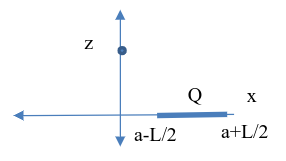
\includegraphics[width=.4\textwidth]{Figures/Figure2-2.png}
        \label{fig:2}
      \end{figure}
    \end{center}

    We know the rod is length $L$, with charge $Q$. This means the linear charge density can be defined as:

    $$\lambda=\frac{Q}{L}$$

    Furthermore, we can refer to the angle between the test charge and point on the rod as $\theta$, and the distance from said point on the rod to the test charge can be called $R$. This yields us the following expression for the $x$-axis:

    \begin{figure}[H]
      \centering
      \tikzset{every picture/.style={line width=0.75pt}} %set default line width to 0.75pt        

\begin{tikzpicture}[x=0.75pt,y=0.75pt,yscale=-1,xscale=1]
%uncomment if require: \path (0,430); %set diagram left start at 0, and has height of 430

%Shape: Axis 2D [id:dp24379060919610995] 
\draw  (189,279.1) -- (447,279.1)(214.8,64) -- (214.8,303) (440,274.1) -- (447,279.1) -- (440,284.1) (209.8,71) -- (214.8,64) -- (219.8,71)  ;
%Shape: Circle [id:dp5068074961038191] 
\draw  [color={rgb, 255:red, 74; green, 104; blue, 226 }  ,draw opacity=1 ][fill={rgb, 255:red, 74; green, 144; blue, 226 }  ,fill opacity=1 ] (212,171.5) .. controls (212,170.12) and (213.12,169) .. (214.5,169) .. controls (215.88,169) and (217,170.12) .. (217,171.5) .. controls (217,172.88) and (215.88,174) .. (214.5,174) .. controls (213.12,174) and (212,172.88) .. (212,171.5) -- cycle ;
%Shape: Rectangle [id:dp4049832220826315] 
\draw  [color={rgb, 255:red, 76; green, 74; blue, 226 }  ,draw opacity=1 ][fill={rgb, 255:red, 74; green, 144; blue, 226 }  ,fill opacity=1 ] (250,272) -- (401,272) -- (401,287) -- (250,287) -- cycle ;
%Straight Lines [id:da700289752662222] 
\draw  [dash pattern={on 0.84pt off 2.51pt}]  (217,171.5) -- (401,272) ;
%Straight Lines [id:da7713004879943914] 
\draw  [dash pattern={on 0.84pt off 2.51pt}]  (214.5,174) -- (250,272) ;
%Curve Lines [id:da724423688563848] 
\draw    (234,180) .. controls (243,182) and (223,204) .. (215,195) ;
%Straight Lines [id:da6170187006178778] 
\draw    (250,272) -- (250,287) ;
%Straight Lines [id:da0940078032787679] 
\draw    (401,272) -- (401,287) ;
%Straight Lines [id:da21330223589749187] 
\draw    (326.5,272.5) -- (326.5,287.5) ;
%Shape: Brace [id:dp2693887070076282] 
\draw   (284,272) .. controls (284,270.21) and (283.11,269.32) .. (281.32,269.32) -- (281.32,269.32) .. controls (278.77,269.32) and (277.5,268.43) .. (277.5,266.65) .. controls (277.5,268.43) and (276.23,269.32) .. (273.68,269.32)(274.82,269.32) -- (273.68,269.32) .. controls (271.89,269.32) and (271,270.21) .. (271,272) ;
%Straight Lines [id:da6088554153847827] 
\draw    (212,171.5) -- (173.58,171.5) ;
\draw [shift={(171.58,171.5)}, rotate = 360] [color={rgb, 255:red, 0; green, 0; blue, 0 }  ][line width=0.75]    (10.93,-3.29) .. controls (6.95,-1.4) and (3.31,-0.3) .. (0,0) .. controls (3.31,0.3) and (6.95,1.4) .. (10.93,3.29)   ;

% Text Node
\draw (222,62.6) node [anchor=south west] [inner sep=0.75pt]    {$z$};
% Text Node
\draw (451,279.4) node [anchor=north west][inner sep=0.75pt]    {$x$};
% Text Node
\draw (216.5,177.4) node [anchor=north west][inner sep=0.75pt]    {$\theta $};
% Text Node
\draw (311,218.35) node [anchor=south west] [inner sep=0.75pt]    {$R$};
% Text Node
\draw (250,290.4) node [anchor=north] [inner sep=0.75pt]    {$a-\frac{L}{2}$};
% Text Node
\draw (401,290.4) node [anchor=north] [inner sep=0.75pt]    {$a+\frac{L}{2}$};
% Text Node
\draw (326.5,290.9) node [anchor=north] [inner sep=0.75pt]    {$a$};
% Text Node
\draw (277.48,264.6) node [anchor=south] [inner sep=0.75pt]    {$dx$};
% Text Node
\draw (169.58,168.1) node [anchor=south east] [inner sep=0.75pt]    {$E_{x}$};


\end{tikzpicture}

      \caption{Supporting Diagram — Problem 2}
      \label{fig:3}
    \end{figure}

    $$E_x=-\int \frac{\sin(\theta)}{4\pi\varepsilon_oR^2}\,dQ$$

    We can express $dq\rightarrow \lambda\,dx$, which gives us:

    $$E_x=-\int \frac{\lambda\sin(\theta)}{4\pi\varepsilon_oR^2}\,dx$$

    Then, if we were to assume $x$ as the horizontal distance from the test charge to the rod, and $z$ as the vertical distance from the test charge to the rod, we may see that: 

    $$\tan(\theta)=\frac{x}{z}$$
    $$z\tan(\theta)=x$$
    $$z\sec^2(\theta)\,d\theta=dx$$

    Taking $R$ into account, we can further simplify our calculation:

    $$\frac{dx}{R^2}=\frac{z\,d\theta}{R^2\cos^2(\theta)}$$

    Again referring to our set up, we know $\cos(\theta)=\dfrac{z}{R}$:

    $$\frac{dx}{R^2}=\frac{d\theta}{z}$$

    Finally, we can use this:

    $$E_x=-\frac{\lambda}{4\pi\varepsilon_o z}\int_{\theta_{a-\frac{L}{2}}}^{\theta_{a+\frac{L}{2}}} \sin(\theta)\,d\theta$$
    $$\frac{\lambda}{4\pi\varepsilon_o z}\left[ \cos(\theta) \right]\Big|_{\theta_{a-\frac{L}{2}}}^{\theta_{a+\frac{L}{2}}}$$

    We can once again refer to the set-up, finding that:

    $$\left\{\begin{array}{l c c}\cos(\theta_{a-\frac{L}{2}})=\frac{z}{\sqrt{z^2+(a-L/2)^2}}\\\cos(\theta_{a+\frac{L}{2}})=\frac{z}{\sqrt{z^2+(a+L/2)^2}}\\\end{array}$$

      Substituting this into our final expression, we get:

      $$\boxed{\frac{\lambda}{4\pi\varepsilon_o}\left( \frac{1}{\sqrt{z^2+(a+L/2)^2}}-\frac{1}{\sqrt{z^2+(a-L/2)^2}} \right)}$$

      \textsc{$z=0$ case:}

      $$\frac{\lambda}{4\pi\varepsilon_o}\left( \frac{1}{a+L/2}-\frac{1}{a-L/2} \right)$$
      $$\frac{\lambda}{4\pi\varepsilon_o}\left( \frac{a-L/2-(a+L/2)}{a^2-(L/2)^2} \right)$$
      $$-\frac{\lambda L}{(4\pi\varepsilon_o)(a^2-(L/2)^2)}$$
      $$-\frac{Q}{(4\pi\varepsilon_o)(a^2-(L/2)^2)}$$

      \textsc{$a>>L$ case:}

      $$\frac{\lambda}{4\pi\varepsilon_o}\left( \frac{1}{\sqrt{z^2+(a+L/2)^2}}-\frac{1}{\sqrt{z^2+(a-L/2)^2}} \right);\quad a\pm L\to 0$$
      $$\frac{\lambda}{4\pi\varepsilon_o}\cancel{\left( \frac{1}{\sqrt{z^2+a^2}}-\frac{1}{\sqrt{z^2+a^2}} \right)}=0$$

      This makes sense, as, logically, if the rod were centered at a point very far away from the test charge, there would be no significant electric field.
    
  \item Calculate the electric potential on the $z$-axis due to a uniformly charged annulus in the $xy$-plane centered at the origin with inner radius $a$ and outer radius $b$. Then find the electric field from the gradient of the potential.

    Let us assume the annulus holds a charge of $q$, with an area $A$. This defines the charge density as:

    $$\sigma=\frac{q}{A}$$

    This gives us:

    $$dq=\sigma dA$$

    If we assume that $i$ and $j$ are the horizontal and vertical distances, respectively, to the test charge from any point on the annulus, and $r=\sqrt{i^2+j^2}$ is the radial distance from the test charge to any point, then we can express the above as:

    \begin{figure}[H]
      \centering
      \tikzset{every picture/.style={line width=0.75pt}} %set default line width to 0.75pt        

\begin{tikzpicture}[x=0.75pt,y=0.75pt,yscale=-1,xscale=1]
%uncomment if require: \path (0,430); %set diagram left start at 0, and has height of 430

%Shape: Donut [id:dp7549476977820966] 
\draw  [color={rgb, 255:red, 74; green, 99; blue, 226 }  ,draw opacity=1 ][fill={rgb, 255:red, 74; green, 144; blue, 226 }  ,fill opacity=1 ,even odd rule][line width=1.5]  (194.66,267.55) .. controls (176.97,262.03) and (171.64,250.2) .. (182.76,241.12) .. controls (193.88,232.03) and (217.24,229.14) .. (234.94,234.65) .. controls (252.63,240.17) and (257.96,252) .. (246.84,261.08) .. controls (235.72,270.17) and (212.36,273.06) .. (194.66,267.55)(164.46,292.22) .. controls (122.11,279.03) and (110.32,249.92) .. (138.13,227.21) .. controls (165.93,204.51) and (222.8,196.79) .. (265.14,209.98) .. controls (307.49,223.17) and (319.28,252.28) .. (291.47,274.99) .. controls (263.67,297.69) and (206.8,305.41) .. (164.46,292.22) ;
%Shape: Axis 2D [id:dp24379060919610995] 
\draw  (189,279.1) -- (447,279.1)(214.8,64) -- (214.8,303) (440,274.1) -- (447,279.1) -- (440,284.1) (209.8,71) -- (214.8,64) -- (219.8,71)  ;
%Shape: Circle [id:dp6435227629373832] 
\draw  [color={rgb, 255:red, 74; green, 144; blue, 226 }  ,draw opacity=1 ][fill={rgb, 255:red, 74; green, 144; blue, 226 }  ,fill opacity=1 ] (202.8,284.55) .. controls (202.8,277.07) and (208.87,271) .. (216.35,271) .. controls (223.83,271) and (229.9,277.07) .. (229.9,284.55) .. controls (229.9,292.03) and (223.83,298.1) .. (216.35,298.1) .. controls (208.87,298.1) and (202.8,292.03) .. (202.8,284.55) -- cycle ;
%Straight Lines [id:da35931985921212983] 
\draw [color={rgb, 255:red, 74; green, 144; blue, 226 }  ,draw opacity=1 ][fill={rgb, 255:red, 255; green, 255; blue, 255 }  ,fill opacity=1 ][line width=1.5]    (253,279) -- (285,279) ;
%Straight Lines [id:da44873433810971197] 
\draw [color={rgb, 255:red, 74; green, 144; blue, 226 }  ,draw opacity=1 ][line width=1.5]    (187,279) -- (253,279) ;
%Straight Lines [id:da19987966215329656] 
\draw  [dash pattern={on 0.84pt off 2.51pt}]  (218.3,91.6) -- (260,226) ;
%Shape: Circle [id:dp9633618470790888] 
\draw  [color={rgb, 255:red, 74; green, 125; blue, 226 }  ,draw opacity=1 ][fill={rgb, 255:red, 74; green, 144; blue, 226 }  ,fill opacity=1 ] (211.3,91.6) .. controls (211.3,89.67) and (212.87,88.1) .. (214.8,88.1) .. controls (216.73,88.1) and (218.3,89.67) .. (218.3,91.6) .. controls (218.3,93.53) and (216.73,95.1) .. (214.8,95.1) .. controls (212.87,95.1) and (211.3,93.53) .. (211.3,91.6) -- cycle ;
%Straight Lines [id:da26890877688664827] 
\draw  [dash pattern={on 0.84pt off 2.51pt}]  (260,226) -- (216,232) ;
%Straight Lines [id:da09923872552730995] 
\draw [draw opacity=0]   (214.8,95.1) -- (216,232) ;

% Text Node
\draw (145,243.4) node [anchor=north west][inner sep=0.75pt]  [color={rgb, 255:red, 255; green, 255; blue, 255 }  ,opacity=1 ]  {$A$};
% Text Node
\draw (271,239.4) node [anchor=north west][inner sep=0.75pt]  [color={rgb, 255:red, 255; green, 255; blue, 255 }  ,opacity=1 ]  {$q$};
% Text Node
\draw (213.4,163.55) node [anchor=east] [inner sep=0.75pt]    {$j$};
% Text Node
\draw (241.15,155.4) node [anchor=south west] [inner sep=0.75pt]    {$r$};
% Text Node
\draw (238,225.6) node [anchor=south] [inner sep=0.75pt]  [color={rgb, 255:red, 255; green, 255; blue, 255 }  ,opacity=1 ]  {$i$};
% Text Node
\draw (214.44,62.6) node [anchor=south east] [inner sep=0.75pt]    {$z$};
% Text Node
\draw (447,281.4) node [anchor=north west][inner sep=0.75pt]    {$x$};

\end{tikzpicture}

      \caption{Supporting Diagram — Problem 3}
      \label{fig:4}
    \end{figure}

    $$dq=\sigma (2\pi i\,di)$$

    We can then define the voltage as:

    $$V=\frac{q}{4\pi\varepsilon_o r}$$
    $$dV=\frac{dq}{4\pi\varepsilon_o r}$$
    $$dV=\frac{\sigma i\,di}{2\varepsilon_o\sqrt{i^2+j^2}}$$

    We can then integrate to find the voltage expression:

    $$V=\frac{\sigma}{2\varepsilon_o}\int_a^b\frac{i}{\sqrt{i^2+j^2}}\,di$$

    Using $u$ substitution, with $u=i^2+j^2$, we get:

    $$V=\frac{\sigma}{\varepsilon_o}\int_{a^2+j^2}^{b^2+j^2}\frac{1}{\sqrt{u}}\,du$$
    $$V=\frac{\sigma}{\varepsilon_o}\left(  \frac{\sqrt{u}}{2}\right)\Big|_{a^2+j^2}^{b^2+j^2}$$
    $$V=\frac{\sigma}{2\varepsilon_o}\left(  \sqrt{j^2+b^2}-\sqrt{j^2+a^2}\right)$$

    We can then find the electric field using the gradient formula:

    $$\vec{E}=-\vec{\nabla}V$$
    $$\vec{E}=-\vec{\nabla}\left(  \frac{\sigma}{2\varepsilon_o}\left(  \sqrt{j^2+b^2}-\sqrt{j^2+a^2}\right) \right)$$
    $$\boxed{\vec{E}=\langle 0, 0, \frac{\sigma}{2\varepsilon_o}\left( \frac{j}{\sqrt{j^2+a^2}}-\frac{j}{\sqrt{j^2+b^2}} \right)\rangle}$$

    Because $j$ simply indicates the $z$ direction, and the vector above is with respect to the $i,j,k$ vectors, we can rewrite this as:

    $$\boxed{\vec{E}=\frac{\sigma}{2\varepsilon_o}\left( \frac{z}{\sqrt{z^2+a^2}}-\frac{z}{\sqrt{z^2+b^2}} \right)\bold{\hat{k}}}$$
    
  \item Consider an infinitely long uniformly-charged solid cylinder of radius $a$ and charge per unit volume $\rho$ surrounded by a coaxial cylindrical shell of radius $b$ and charge per unit area of $\sigma$. Take the axis of the cylinders as the $z$-axis.

    \begin{enumerate}

      \item Calculate the electric field everywhere in space

        We must calculate the electric field in three different cases:

        \begin{enumerate}

          \item The radius $r<a$ (that is, in the cylinder)

            First, we must find the electric field inside of the cylinder, since we can not assume it is a cylinder. We do this with the following set up:

            $$\int \vec{E}\cdot dA=\frac{q_{enc}}{\varepsilon_o}$$

            Since the electric field is a function of $r$, it can be removed from the integral:

            $$\vec{E}\int dA=\frac{q_{enc}}{\varepsilon_o}$$

            The area integral, with $l$ being the length of the cylinder, gives us:

            $$\vec{E}(2\pi rl)=\frac{q_{enc}}{\varepsilon_o}$$

            The charge enclosed is simply the charge density of the cylinder is the charge density multiplied by the volume:

            $$\vec{E}(2\pi rl)=\frac{\rho(\pi r^2l)}{\varepsilon_o}$$

            We then divide over to get:

            $$\boxed{\vec{E}=\frac{\rho r}{2\varepsilon_o}}$$

          \item The radius $a<r<b$ (that is, in between the cylinder and shell)

            We can find the electric field in a similar process to the above:

            $$\vec{E}\int dA=\frac{q_{enc}}{\varepsilon_o}$$
            $$\vec{E}(2\pi rl)=\frac{\rho(\pi a^2 l)}{\varepsilon_o}$$
            $$\boxed{\vec{E}=\frac{\rho a^2}{2r\varepsilon_o}}$$

          \item The radius $r>b$ (that is, outside of the coaxial cable)

            Again, we repeat a similar process:

            $$\vec{E}\int dA=\frac{q_{enc}}{\varepsilon_o}$$
            $$\vec{E}(2\pi rl)=\frac{\rho(\pi a^2l)+\sigma(2\pi bl)}{\varepsilon_o}$$
            $$\boxed{\vec{E}=\frac{\rho a^2+2b\sigma}{2r\varepsilon_o}}$$

        \end{enumerate}

      \item Also calculate the potential as a function of the distance from the axis, taking the potential to be zero on the $z$-axis.

        To find the voltage, we must integrate the three above cases:

        \begin{enumerate}

          \item $r<a$

            $$V=-\int \frac{\rho r}{2\varepsilon_o}\,dr$$
            $$=-\frac{\rho}{\varepsilon_o}\int r\,dr$$
            $$\boxed{V_{r<a}=-\frac{r^2\rho}{4\varepsilon_o}}$$

          \item $a<r<b$

            $$V=-\int \frac{\rho a^2}{2r\varepsilon_o}\,dr$$
            $$=-\frac{\rho a^2}{2\varepsilon_o}\int_a^r r^{-1}\,dr$$
            $$=-\frac{\rho a^2}{2\varepsilon_o}\ln\left(\frac{r}{a}\right)$$

            We then need to add the previous voltage:

            $$\boxed{V_{a<r<b}=-\frac{\rho a^2}{2\varepsilon_o}\ln(\frac{r}{a})-\frac{\rho a^2}{4\varepsilon_o}}$$

          \item $r>b$

            $$V=-\int \frac{\rho a^2+2b\sigma}{2r\varepsilon_o}\,dr$$
            $$=-\frac{\rho a^2+2b\sigma}{2\varepsilon_o}\int_b^r r^{-1}\,dr$$
            $$=-\frac{\rho a^2+2b\sigma}{2\varepsilon_o}\ln\left( \frac{r}{b} \right)$$

            We then need to add the previous voltage:

            $$\boxed{V_{r>b}=-\frac{\rho a^2+2b\sigma}{2\varepsilon_o}\ln(\frac{r}{b})-\frac{\rho a^2}{2\varepsilon_o}\ln(\frac{b}{a})-\frac{\rho a^2}{4\varepsilon_o}}$$

        \end{enumerate}

    \end{enumerate}
    
  \item The electric field for two charged concentric spherical shells is given by

    $$\left\{\begin{array}{c c} 0, & r<a\\ \bold{\hat{r}}A_1/r^2, & a< r< b\\ \bold{\hat{r}}A_2/r^2, & r>b \end{array}$$

      Where $A_1=5\times 10^6\left[ \frac{\si{\newton\meter\squared}}{\si{\coulomb}} \right]$, $A_2=-3\times10^6\left[ \frac{\si{\newton\meter\squared}}{\si{\coulomb}} \right]$, $a=.25[\si{\meter}]$, and $b=.45[\si{\meter}]$. Find the surface charge densities $\sigma_a$ and $\sigma_b$ on the two shells.

    We can apply Gauss's law to help us find the electric field:

    \begin{enumerate}

      \item $r<a$

        $$\vec{E}(4\pi r^2)=\frac{4\pi r^2\sigma_a}{\varepsilon_o}$$
        $$\sigma_a=\varepsilon_o\vec{E}$$

        $\vec{E}=0$ in this case, so it does not provide enough information.

      \item $a<r<b$

        $$\vec{E}(4\pi r^2)=\frac{4\pi a^2\sigma_a}{\varepsilon_o}$$
        $$\sigma_a=\vec{E}\frac{r^2}{a^2}\varepsilon_o$$
        $$=\frac{A_1}{a^2}\varepsilon_o$$
        $$=\frac{5\cdot10^6}{(.25)^2}(8.85\cdot10^{-12})$$
        $$\boxed{\sigma_a=7.08\cdot10^{-4}\left[ \frac{\si{\coulomb}}{\si{\meter\squared}} \right]}$$

      \item $r>b$

        $$\vec{E}(4\pi r^2)=\frac{4\pi a^2\sigma_a+4\pi b^2\sigma_b}{\varepsilon_o}$$
        $$\vec{E}=\frac{a^2\sigma_a+b^2\sigma_b}{r^2\varepsilon_o}$$
        $$\sigma_b=\frac{A_2\varepsilon_o-a^2\sigma_a}{b^2}$$
        $$\boxed{\sigma_b=-3.496\cdot10^{-4}\left[ \frac{\si{\coulomb}}{\si{\meter\squared}} \right]}$$

    \end{enumerate}
    
\end{enumerate}

\end{document}

